\documentclass[12pt]{article}
\usepackage[spanish]{babel}
\usepackage[margin = 21mm]{geometry}
\usepackage{amsmath, amssymb, amsfonts}
\usepackage{parskip}
\usepackage{multicol}
\usepackage{graphicx}

\usepackage[proportional,scaled=1]{erewhon}
\usepackage[erewhon,vvarbb,bigdelims]{newtxmath}
\usepackage[T1]{fontenc}
\renewcommand*\oldstylenums[1]{\textosf{#1}}

\begin{document}
	%Portada
    \begin{titlepage}
        \centering
        \vspace{2.7cm}
        {\Huge \textbf{Universidad Autónoma del Estado de México}\par}
        \vspace{0.9cm}

        {\Huge \textbf{Facultad de Ciencias}\par}
        \vspace{0.9cm}

        {\Huge \textbf{Licenciatura en Matemáticas}\par}
        \vspace{0.9cm}

        {\huge \textbf{Topología}\par}
        \vspace{0.9cm}

        {\huge \textbf{Profesor:}\par}
        \vspace{0.3cm}
        {\huge \textsl{Enrique Castañeda Alvarado}}\par
        \vspace{1.4cm}

        {\huge \textbf{Proyecto 3: \\ La caprichosa forma de globión}\par}
        \vspace{1.4cm}

        {\huge \textbf{Alumno:}\par}
        \vspace{0.3cm}
        {\huge \textsl{Santana Reyes Osmar Dominique}}\par
        \vspace{0.9cm}

        {\huge \textbf{No. de cuenta:} 2125197 \par}
        \vspace{0.7cm}
        \vfill
        \raggedleft{\LARGE Fecha de Entrega: 10 de junio de 2022}\par         %Alinear a la derecha
    \end{titlepage}

	\begin{multicols}{2}

		La topología es una rama de las matemáticas que estudia las propiedades de figuras o espacios que permanecen invariantes, bajo transformaciones continuas. Estas propiedades suelen ser globales, lo cual hace que la topología se distinga de otras ramas de las matemáticas cuyo estudio es puntual y se sujeta a ciertas condiciones, como la geometría euclidiana a los postulados de Euclides. Esta rama es de reciente creación, al menos de manera formal, pues se pueden rastrear sus orígenes a finales del siglo XIX en el \textit{Analysis Situs} de Leibniz, mediante el cual buscaba ofrecer un estudio más cualitativo del espacio. Hoy en día, la topología es una disciplina que requiere varios estudios en diversos temas, uno de estos son las superficies. 

		En el libro \textit{La caprichosa forma de Globión}, Alejandro Illanes Mejía tiene la intención de presentar al lector el estudio de las superficies y sus aplicaciones en la vida real, mediante una historia ficticia en la que cierta cantidad de personas son transportadas a un planeta que posteriormente es llamado \textit{Globión}. Después de esto, las personas se encuentran en una época de ``oscurantismo'' y guerras, que impiden el desarrollo de las ciencias y las artes. Una vez terminada esta época, se encuentran libros que fueron elaborados en la Tierra y contienen una gran cantidad de conocimientos que causan un gran desarrollo en la población. Tiempo después un grupo de científicos comienza un proyecto para mapear el planeta Globión, del cual no se sabe qué forma tiene. Al principio, todos pensaban solamente en hacer mapas de las distintas regiones de globión hasta cubrirlo completamente, pero al ser un proceso muy tardado empiezan a investigar las posibles formas que podría tener Globión.

		De esta manera, se empiezan a exponer varias ideas y conceptos que tienen su fundamento en la topología. La primera es que dos superficies son equivalentes si una se puede deformar hasta ser como la otra, lo cual formalmente está representado por los \textit{homeomorfismos}. Además, para lograr esta equivalencia no solo es posible deformar la superficie, si no que también se permite ``recortar'' cierta sección de la superficie, y manipularla con la condición de que al final se vuelvan a unir los bordes que fueron separados. Esto tiene su fundamento en los espacios cociente, que permiten establecer homeomorfismos entre dos espacios en los que pareciera que uno fue ``dividido'' y manipulado hasta ser como el otro, o por el contrario, uno se ``pegó'' de cierta forma, con una sección de si mismo para ser como el otro. Como ejemplo de lo anterior, se puede pensar en una esfera que es perforada y se estira este agujero hasta obtener un objeto plano, que puede ser estirado de cuatro puntos para convertirlo en un plano.

		Otra idea que se explica en el libro, es que toda región puede cubrirse con un polígono, que a su vez se puede dividir en triángulos. A primera vista, esto pareciera ser una manera de facilitar la comprensión de las distintas operaciones que se hacen a lo largo del libro, pero incluso esto es un concepto topológico conocido como \textit{base}. Una base es un conjunto de ``piezas'' de un espacio con las que es posible representar cualquier región de este espacio, ya sea uniendolas o sobreponiendolas. En este caso, la base puede estar formada por todos los triángulos que sea posible trazar en la superficie de Globión.

		Posteriormente, se indaga en la posibilidad de simplificar las superficies, es decir, si se encuentran varias de estas que resultan ser equivalentes, entonces hallar una forma fundamental en la que todas puedan ser convertidas y asi poder diferenciarlas de otras con las que no lo son. Resulta que si es posible, y se llega a la siguiente conclusión: ``\textit{Toda superficie es una esfera con chipotes en forma de bonete, rosca o botella de Klein}''. 

		\begin{center}
			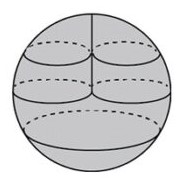
\includegraphics[width=45mm]{bonete.jpg}

			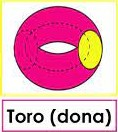
\includegraphics[width=45mm]{toro.jpg} 

			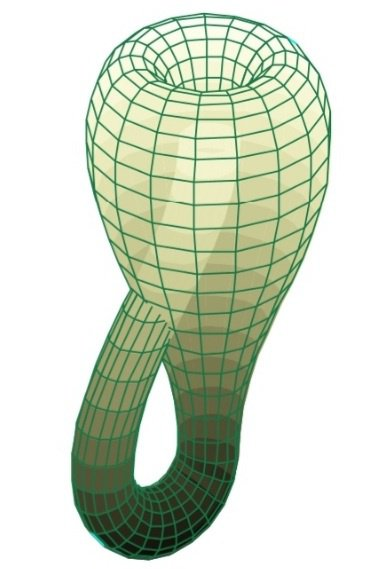
\includegraphics[width=45mm]{Klein.jpg}
		\end{center}

		En el resto del libro, se explican otras propiedades de las superficies, que también son aplicables a los espacios topológicos, además de propiedades geométricas muy interesantes y un poco de teoría de gráficas.

		Illanes Mejía expone de una manera clara todas las ideas que se usan para describir las superficies y lo que se puede hacer con ellas, hay muchos dibujos que ayudan al lector a comprender todo lo abordado. Además, la trama va fluyendo de manera adecuada sin perder el hilo de la historia ni concentrarse demasiado en el tema de las superficies. Al final, el autor usa algunas herramientas matemáticas que tal vez el lector no comprenda del todo, pero esto no perjudica la lectura ni la comprensión de las ideas principales. 

		Para concluir, se puede decir que la topología es una rama muy amplia de las matemáticas que tiene poco de haber aparecido, pero que ofrece varias oportunidades de estudio. Una muestra de ello es el tema de las superficies que se tratan en el libro, que es solo una de las tantas cosas que hay en la topología. 

		\textbf{Referencias}

		Romero Contreras Arturo. (2020). \textit{Entrevista con Luciano Boi ¿Qué es la topología?}. Redalyc. https://www.redalyc.org/journal/594\\/59463123009/html/

		Macho Stadler Marta. (2002, febrero). \textit{¿Qué es la topología?}. SIGMA. https://www.ehu.eus/~mtwmastm/sigma20.pdf
	\end{multicols}
\end{document}